\scanpage{60}
% archive sheet number: 59
\margin{[\unsure{dans ce cas} \deleted{\unsure{les objets} $(x,\unsure{\zeta|\xi})$ \unsure{de $A_c$}} \inserted{$X$ est une catégorie, \unsure{définie par les|désignons par les}} \unsure{morphismes de} $X$: \unsure{les couples} $(c,\zeta)$, où \unsure{$c$ est une chaine saturée de $x_0$ à $x_n$} et $\zeta\in A_c$]}
\unsure{est|une} \uline{associative}. L'étendant par $0$ si \deleted{$\unsure{A_c}$ et} $\unsure{c'|c}$ et $c$ ne sont pas composables, la somme des $A_c$ devient un anneau $A^*$ [en général non commutatif], \inserted{\uline{gradué} par la longueur des chaines}, la somme des $A_x$ \unsure{devient|donne} un sous-anneau (commutatif), \unsure{soit|savoir} $A^0$.

$A^1$ est la somme des $A_{[x_0,x_1]}$, soit $\Theta$ l'élém de $A^1$ dont les composantes sont $1_{[x_0,x_1]}$.

\deleted{Quel est $\Theta^2$ ?} On a
\[
\Theta^2=\sum_{\substack{(x_0,x_1)\\(\unsure{x_0|y_0},y_1)\\\text{chaines}\\\text{saturées}}}
1_{[x_0,x_1]}\cdot1_{[y_0,y_1]}
=\sum_{\substack{[x_0,x_1,x_2]\\\text{chaines}\\\text{saturées}}}\cdot1_{[x_0,x_1,x_2]}
\]

On va maintenant diviser par l'idéal \inserted{bilatère} engendré par $\Theta^2$, \deleted{[\unsure{ce qui signifie aussi}, \unsure{semble-t-il}, \unsure{que l'on impose que}}

\uline{$\unsure{u_1+\partial u_2}$}
En dim $0$ et $1$, cela ne tue rien, en dim $2$ il faut \unsure{coégaler} les
\[
\sum_{\substack{x_1\\\text{\unsure{intermédiaire} à}\\a\ \text{et}\ b\\(\text{\unsure{où}}\ \delta(a,b)=2)}}\varphi
\]

\figure{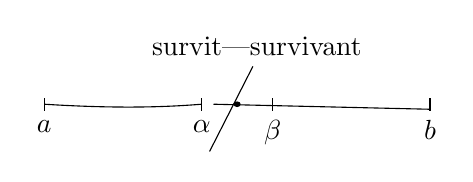
\begin{tikzpicture}[x=1cm,y=.8cm]
\draw (0,0)..controls (.9,-.07) and (1.5,-.05)..(2,0);\draw (2.15,0)--(4.9,-.08);
\foreach \x in {0,2,2.9,4.9}{\draw (\x,-.1)--(\x,.1);}
\node[below] at (0,-.1) {$a$};\node[below] at (2,-.1) {$\alpha$};\node[below] at (2.9,-.1) {$\beta$};\node[below] at (4.9,-.1) {$b$};
\fill (2.45,0) circle (.045);\draw (2.1,-.75)--(2.65,.6);\node[above] at (2.7,.62) {\unsure{survit|survivant}};
\end{tikzpicture}}
\diagram{\begin{tikzcd}[ampersand replacement=\&]x_0\arrow[r]\&x_n\end{tikzcd}}
\diagram{\begin{tikzcd}[ampersand replacement=\&]
A_{[a-\alpha,\delta,\beta,\ldots b]}\\
A_{[a-\alpha]}\otimes_{\substack{A_\alpha\ \text{\unsure{complété|completé}}\\\text{par}\ \beta}}A_{[\beta\ldots\unsure{b}]}\arrow[u,"\varphi_{\unsure{\delta|v}}"]
\end{tikzcd}}
\diagram{\begin{tikzcd}[ampersand replacement=\&]
A_{[a-\alpha]}\&A_{[\beta-b]}\\
A_{[\alpha]}\arrow[u]\arrow[u,bend left=30]\&A_{[\beta]}\arrow[u]
\end{tikzcd}}
[$A_\alpha$ \unsure{complété|completé} par $\beta$]
